\chapter{Sistema de linealización}
\label{ch:linealizacion}

Para realizar la linealización de la expresión exponencial de la corriente $\ i_{pv} $ del modelo del panel se implementa una función logarítmica, dentro de los algoritmos de calculo se tiene el de CORDIC, este permite realizar una aproximación de la función de manera recursiva mediante cierta cantidad de iteraciones, para el caso del linealizador se utiliza el método hiperbólico para realizar el calculo de la operación logaritmo natural, este algoritmo requiere de una tabla (Look-up table) con valores pre-cargados. 

El rango de convergencia para este algoritmo es de $\ 0.106843 < T < 9.35947 $ donde $\ T $ es el argumento del logaritmo natural, el valor máximo de $\ T $ para el panel previamente escogido de 0.58A esta es la corriente en condiciones máximas para el panel, debido a esto se puede desplazar el intervalo que se tiene para los argumentos, este se divide entre una constante $\ C = 16$ y se desplaza $\ 0.00667769 < T < 0.58496687 $, esto se realizo debido a que se pueden dar valores de corriente mas bajos que 0.106843A. Esta constante C se debe compensar en el logaritmo, y se logra con la siguiente igualdad: 

\begin{equation} \label{eq:ej1}
  Ln \left( T \right)
  = Ln \left( 16T \right) - Ln\left( 16 \right) 
\end{equation}  

  

\section{Algoritmo de CORDIC en software}
 
Para comprobar el debido funcionamiento del este algoritmo se crea un programa de alto nivel en Python.  


\begin{figure}[H]
  \centering
    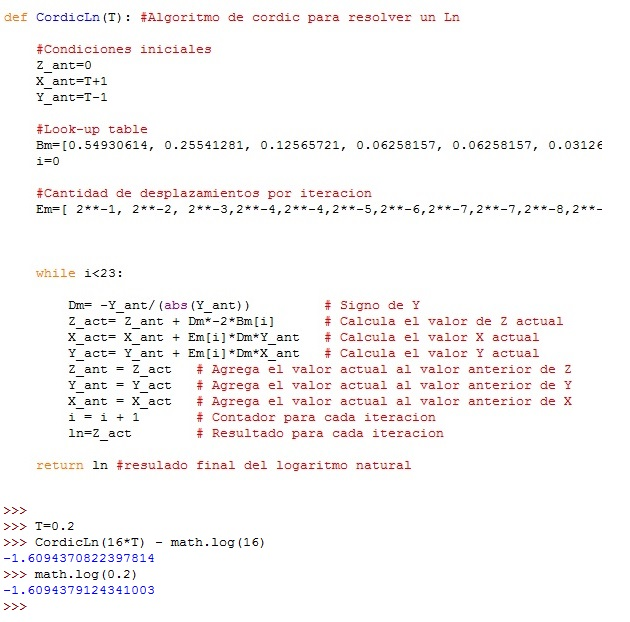
\includegraphics[scale=0.6]{./Progra_Cordic.jpg}
    \rule{35em}{0.5pt}
  \caption[Algoritmo de CORDIC en Python]{Algoritmo de CORDIC en Python  }
  \label{fig:Python}
\end{figure}


En la figura \ref{fig:Python} se observa el programa realizado para la verificación del algoritmo, para este se utilizan las ecuaciones del marco teórico descritas con anterioridad, también se comprueba el cambio en el rango de calculo con el escalado del argumento por 16. 

Para simplificar el diseño del hardware se realizan cambios en las ecuaciones originales, se cambia la resta del valor actual de Z por una suma, y se incluye el signo en la LUT de Z, el resultado final del algoritmo se debe multiplicar por 2, sin embargo este escalado se puede realizar en la LUT, esto para evitar la multiplicación, esto se comprueba en el programa de la figura \ref{fig:Python}.  


\section{Arquitectura del algoritmo de CORDIC}

El diseño de este algoritmo se basa en la arquitectura segmentada, de manera que se almacenan varios datos a la vez, sin embargo se debe tener buena sincronización para evitar datos erróneos a través del proceso de calculo. 

\begin{figure}[H]
  \centering
    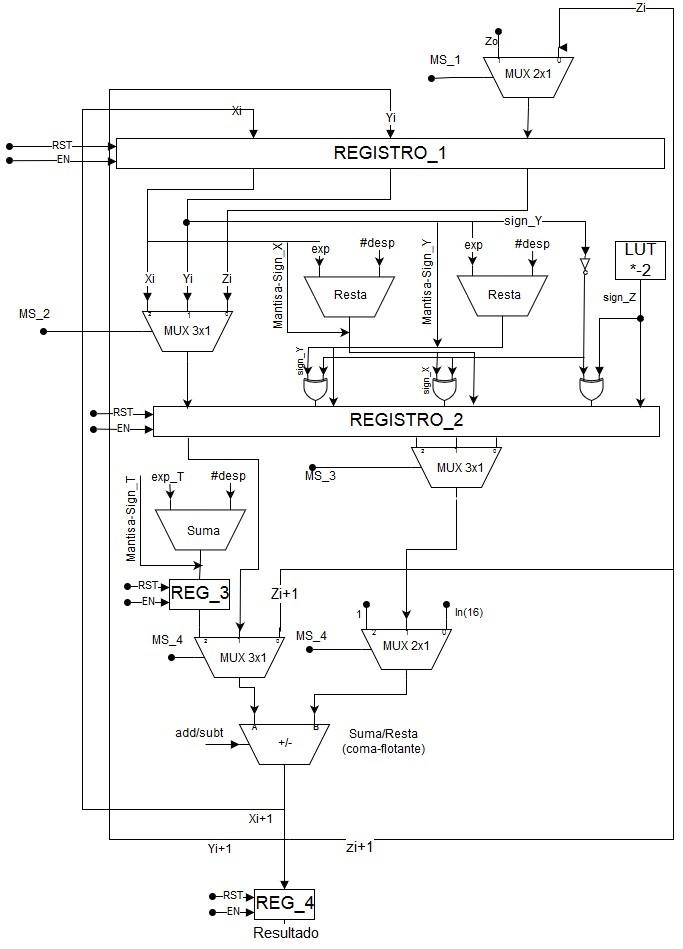
\includegraphics[scale=0.6]{./CORDICLN.jpg}
    \rule{35em}{0.5pt}
  \caption[Algoritmo de CORDIC en hardware]{Algoritmo de CORDIC en hardware  }
  \label{fig:CORDICLN}
\end{figure}

En la figura \ref{fig:CORDICLN} se puede observar la arquitectura diseñada para el algoritmo de CORDIC, esta utiliza el formato IEEE 754, se trabaja en punto flotante para una mejor precisión tanto en las operaciones como el resultado final. 

Esta etapa inicia con la carga de las condiciones iniciales, donde $\ Z_0 $ contiene un valor inicial cero, para el valor inicial de $\ X_0 $ y $\ Y_0 $ primeramente se aplica el escalado  16*T,
este escalado se puede representar como un desplazamiento $\ 2^{-4} $, por lo tanto este movimiento en punto flotante se traduce como una suma de 4 en el exponente de $\ T$, posteriormente se realizan las siguientes operaciones en punto flotante,  $\ X_0 = T + 1 $ y $\ Y_0 = T - 1 $, estas tres constantes dan inicio al proceso de calculo de manera iterativa, por lo que se requiere almacenarlas en un registro en la primera etapa de segmentación $\ \left(Registro 1 \right) $, los nuevos estados se deben calcular uno por uno, esto porque el circuito para el sumador-restador en punto flotante requiere de mucha área, para el calculo de $\ Xi $ se requiere un restador en punto fijo para el exponente de $\ Y_0 $ , para el nuevo valor de $\ Y_i $ se utiliza un restador para el exponente de $\ X_0 $ y para $\ Z_i $ se requiere una ROM con valores previamente cargados $\ \left(LUT \right) $. Estas operaciones "$\ X_i , Y_i $"  involucran el signo de "$\ Y_0 $" invertido, sin embargo se debe comparar como se observa en la siguiente tabla: 

\begin{table}[H]
\centering
\caption{Tabla de signo}
\label{Table:Signo}
\begin{tabular}{|c|c|c|c|c|c|c|}
\hline
Sign $\ X_0 $ & Sign $\ Z_0 $  & Sign $\ Y_0 $ & Sign $\ \sim Y_0 $  & Sign $\ X_i $ & Sign $\ Z_i $  & Sign $\ Y_i $      \\ \hline

\begin{tabular}[c]{@{}c@{}} 0
\end{tabular}  & 0 & 0   & 1   & 1 & 1 & 1       \\ \hline

\begin{tabular}[c]{@{}c@{}} 0
\end{tabular} & 0 & 1   & 0  & 0 & 0 & 1       \\ \hline

\begin{tabular}[c]{@{}c@{}} 0 
\end{tabular} & 1 & 0   & 1 & 1 & 0 & 1\\ \hline
\begin{tabular}[c]{@{}l@{}} 0
\end{tabular} & 1 & 1   & 0  & 0 & 1 & 1   \\ \hline

\begin{tabular}[c]{@{}l@{}} 1
\end{tabular} & 0 & 0   & 1 & 0 & 1 & 1   \\ \hline

\begin{tabular}[c]{@{}l@{}} 1
\end{tabular} & 0 & 1   & 0  & 1 & 0 & 1   \\ \hline

\begin{tabular}[c]{@{}l@{}} 1
\end{tabular} & 1 & 0   & 1  & 0 & 0 & 1   \\ \hline

\begin{tabular}[c]{@{}l@{}} 1
\end{tabular} & 1 & 1   & 0 & 1 &  1 & 1    \\ \hline


\end{tabular}
\end{table}

a partir de la tabla \ref{Table:Signo} se extrae el circuito de comparación de signo, este es diseñado con compuerta \nt{XOR} que poseen el mismo comportamiento de la tabla.  

Se requiere de dos Look-up tables "LUT", la primera almacena los valores de $\ -2arctanh \left( 2^{-i} \right) $ según sea para cada iteración,  la segunda tabla almacena los desplazamientos de cada iteración, esto debido a que las iteraciones 4 y 13 repiten desplazamientos como se menciona en el marco teórico. 

El proceso para el calculo de las variables no se puede realizar de manera simultanea, ya que solo se cuenta con un sumador punto flotante, se almacena las variables iniciales y las modificadas en el \nt{Registro 2}, la secuencia de calculo toma primeramente los valores y calcula $\ X_i $ y almacena el resultado en el \nt{Registro 1}, posteriormente se procede con el calculo de $\ Y_i $ y se almacena en el \nt{Registro 1}, por ultimo se calcula el valor de $\ Z_i $, concluida la suma se almacena en el \nt{Registro 1}, este proceso se hace de manera iterativa, una vez finalizada la cuenta de 15 iteraciones, se realiza la resta $\ Z_i - Ln\left(16\right) $ para contrarrestar el efecto del escalado aplicado al argumento$\ \left(T\right) $ al inicio del calculo, por ultimo el resultado final $\ Z_i $ se almacena en el \nt{Registro 4}.

\section{Control}

\begin{figure}[H]
  \centering
    \includegraphics[scale=0.48]{./MaquinaL.png}
    \rule{35em}{0.5pt}
  \caption[Maquina de estados finitos para la arquitectura de CORDIC]{Maquina de estados finitos para la arquitectura de CORDIC   }
  \label{fig:FSML}
\end{figure}

\section{algoritmo de CORDIC en Verilog}


\section{Simulación del algoritmo de CORDIC}

\begin{figure}[H]
  \centering
    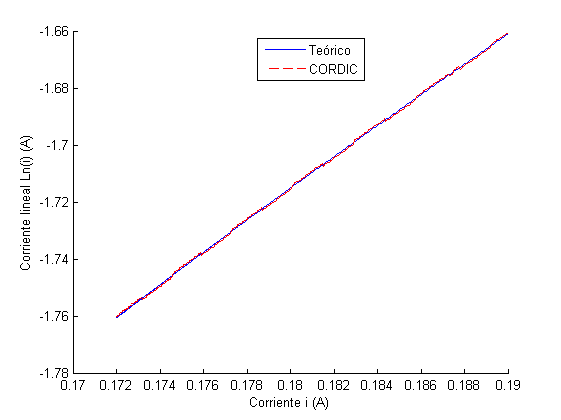
\includegraphics[scale=0.7]{./grafico1.png}
    \rule{35em}{0.5pt}
  \caption[Datos lineales de corriente ipv]{Datos lineales de corriente $\ i_{pv}$ para un PV: teóricos y experimentales   }
  \label{fig:lineal}
\end{figure}









    